\section{A Logical Architecture for an Update Mechanism}
The proposed architecture must identify the core components of a decentralized update system and define how the various new events (Update Proposals, Votes, Delegations, Update Activations etc.) are incorporated into the blockchain system and finally describe the interactions between these components.

\begin{figure}[H]
    \caption{A Logical Architecture for a Decentralized Update Mechanism}
    \centering
    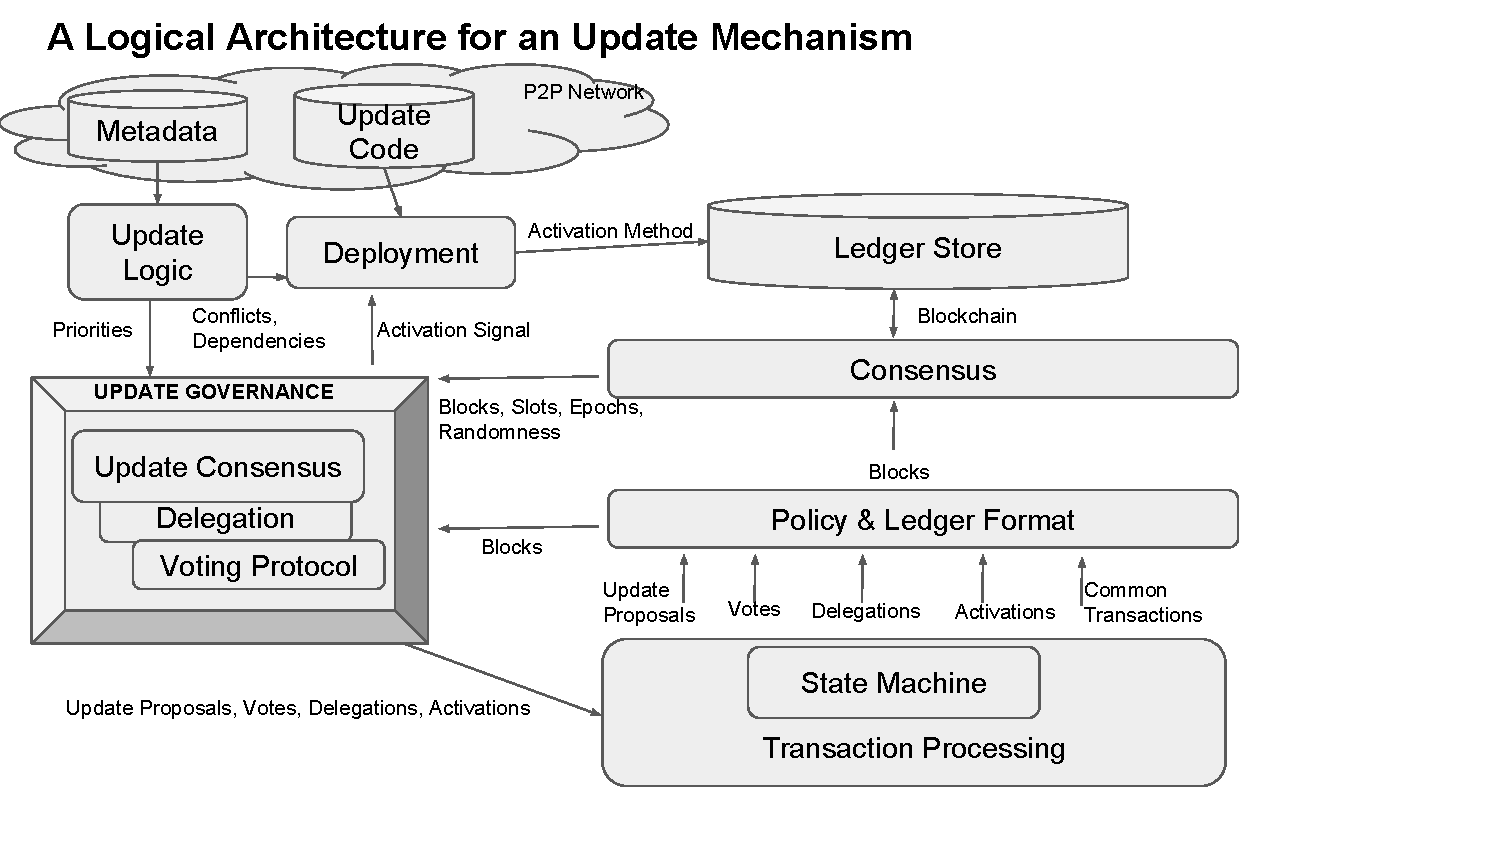
\includegraphics[width=0.9 \columnwidth,keepaspectratio]{figures/logical_architecture_v3.pdf}
    \label{logarch}
\end{figure}

In figure \ref{logarch}, we depict a logical architecture that incorporates a software update mechanism in a distributed ledger. In this figure, we can see that the set of events flowing into the ledger system has been enhanced. Apart from the traditional transactions, which deal with the transfer of value between stakeholders and trigger changes to the global state, now we can see other events such as \emph{Update Proposals}, \emph{Votes}, or even \emph{Vote Delegations} and \emph{Activation events} being generated from the \emph{Update Governance} component and entering the ledger system.

Our primary goal is to store all these new events that pertain to the update mechanism, within the ledger itself, as an immutable record of historical events. To this end, these new events are transformed to special types of transactions and as such, have to go through the rigorous transaction validation process, performed by each node of the network. This is depicted at the Transaction Processing component, where all the logic for what makes a legitimate transaction is implemented.

Ordinary transactions change the global state of value distribution but in the case of smart contracts \cite{smart-contracts} can also change the state of smart contract persistent data by triggering the execution of smart contract code. Update events do not change the global state in the same sense; however, one can imaging an ''Update Proposal state'', representing the number of Update Proposal submitted by a user. Similarly, one could also define a ''Voting state'' representing the votes gathered by each proposal.

Transactions are included into blocks by the Policy and Ledger Format component and these newly generated blocks are passed on to the next layer. The consensus component is where we achieve consensus on what block is legitimate and which blockchain branch is the legitimate one and a new block can be attached to it safely. Regardless of the ''type'' of the consensus protocol (either proof-of-work, or proof-of-stake) the consensus rules that guide the block validation logic must be enhanced to incorporate the new events (i.e., transaction types) that are to be stored in the ledger. As we depict in the figure, the ultimate destination of all types of events is the distributed ledger, which serves as the \emph{single version of the truth} for the updating history of the system.

In particular, for the Cardano \cite{Cardano} case one has to consider the possible enhancements necessary for the Ouroboros family of protocols \cite{C:KRDO17}. Apart from the block validation affecting the consensus rules, one has to take into account the possible impact from the protocols from the \emph{Update Governance} component depicted in the figure.

Update Governance is the component in the architecture that enables a truly decentralized and democratic updating mechanism. It allows all users to freely vote on update proposals and then considers the stake distribution for forming the final result. This is achieved via a secure \emph{voting protocol} that must be tightly integrated with the Blockchain consensus protocol. Moreover, for these users that might be owners of stake but lack the skills and expertise to vote for or against a software update proposal, a \emph{voting delegation protocol} must be in place. This will enable the delegation of the voting right to some other user (regardless of his/her stake), a so-called \emph{expert}, that will assume the voting task in his/her stead. The ultimate goal of the voting and delegation protocols is all the participating users to reach at an \emph{update consensus}. In other words, to reach a common agreement on the update proposal priorities and on the evolution roadmap of the ledger system. Voted update proposals eventually, must be deployed to the system and become \emph{adopted updates}, which are activation events that are stored in the ledger, as well.

\todo{Nikos: We need to decide if we will store activation events in the ledger}

The \emph{Update Logic} component, handles the rules that will guarantee a seamless and versatile activation of software updates into the ledger system. More specifically this component implements the necessary ''logic'' for conflict resolution and secures the updating mechanism from updates that might lead the system to an unstable state. In addition, it supports the correct enforcement of update dependencies and prevents update patches to be installed, if required previous patches are missing. Finally, it implements the notion of \emph{Update Policies}, which differentiate speed of deployment and method of deployment based on: a) the type of change (bug -fix or change request), b) the part of the system that is affected by the change (consensus rules impact, or only software impact) and c) the urgency of the change (severity level). The method of deployment determines the actual mechanism that will be used in order to activate an update in the ledger system. It is executed by the \emph{Deployment} component depicted in the figure. For protocol changes one must consider the most appropriate method for such a deployment and choose among a set of well-known practices such as hard-forks and soft-forks but also from more niche techniques, such as velvet-forks \cite{velvet} and the sidechains mechanism \cite{sidechains}.

\todo{Nikos: I am not sure that hard/soft/velvet forks are a deployment method. Sidechains is. I think there are just different types of consensus rules change}

For all these to work, the Update Logic component must be based on an appropriate set of \emph{Update Metadata}. These metadata must obligatory accompany each submitted Update Proposal and sufficiently describe the change, its expected benefit, its type, its urgency for deployment, its possible conflicts with other updates and many more. In addition to the metadata, every update proposal must be accompanied by the update patch that comprises the actual code to be installed. Both of these two, the metadata and the code, cannot be stored in the ledger, due to their sizing requirements. In order to satisfy the requirement for a truly decentralized update mechanism, one should avoid to store these data into any type of centrally owned servers (e.g., into the cloud). One should consider the use of a P2P file storage or database solution, with \emph{content addressable} \cite{content-addressable} storage capabilities. Moreover, the proposed solution  must guarantee the security of the downloaded software, as well as the authenticity with respect to the original update proposal.
